In this section, we analyze region-wide trends in accessibility losses for the case study area. We first analyze each of the 12 socio-economic groups used in practice for the case study region~\cite{ory_personal_2013}. These socio-economic groups correspond to all combinations of four income classes (Table~\ref{tab:incomes}),
and three classes of automobile availability in the household (zero automobiles, fewer automobiles than household members that work, as many or more automobiles than household members that work). Each data point for analysis represents a trip by a person of a household from one of these segments, who is modeled as an agent in the transportation model.
Expected losses are computed by taking an average of the accessibility losses for people within a given group and region for each earthquake event, weighted by the events' corresponding occurrence rates. Expected losses for people from each of the 12 groups and 1454 TAZs are shown in Figure~\ref{fig:acc_by_segment}. 

In addition to looking at average accessibility loss, we can compute an accessibility exceedance curve for a given group or region. By using equation~\ref{eq:exceedance} to compute exceedance rates for multiple accessibility loss thresholds, we can produce results like those in Figure~\ref{fig:acc_by_TAZ_and_income}. These curves show, for a given group, the annual rate with which a given accessibility decrease will be observed (when considering random future occurrences of earthquakes and damage). Several observations can be made from these results. 


%maps of socio-economic groups
 
\begin{figure*}[ht!]
    \centering
    \includegraphics[height=7in]{FIGS/accByGroup.pdf}
\caption{Expected changes in accessibility per person per day for each combination of income class and car ownership group. The darker the color, the greater the losses in accessibility. Each row of figures corresponds to an income class and each column corresponds to a class of car ownership). }% (no cars, workers $<$ cars , workers $\geq$ cars }
%: a) low income, no cars, b) low income, workers $<$ cars, c) low income, workers $\geq$ cars, d) medium income, no cars, e) medium income, workers $<$ cars, cf) medium income, workers $\geq$ cars, g) high income, no cars, h) high income, workers $<$ cars, i) high income, workers $\geq$ cars, j) very high income, no cars, k) very high income, workers $<$ cars, l) very high income, workers $\geq$ cars}
\label{fig:acc_by_segment}
\end{figure*}


\begin{figure}[!htb]
\centering
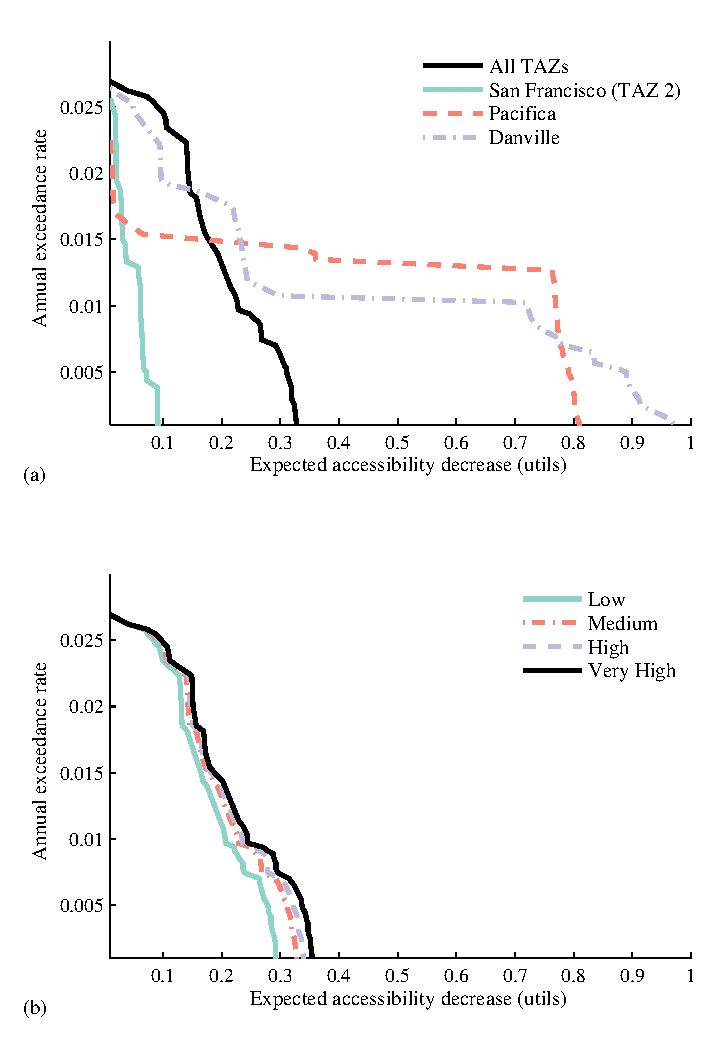
\includegraphics[width=4in]{FIGS/equity_acc_loss_curves.eps} 
\caption{Accessibility annual loss exceedance curve with a comparison by (a) case study TAZs and average over all TAZs and (b) income class; all curves are for medium income households with fewer cars than workers.}
\label{fig:acc_by_TAZ_and_income}
\end{figure}


\begin{table}
\caption{Income class definitions for the case study region, as defined by the local planning organization, the MTC~\cite{ory_personal_2013} and also translated to current 2014 USD using the consumer price index.}
\centering
\begin{tabular}{c|c|c}
\textbf{Income class}           & \textbf{Income range, 1989 USD} & \textbf{Income range, 2014 USD} \\
\hline
Low & $<$ \$25,000 & $<$ \$47,334\\
Medium &  \$25,000 - \$45,000 & \$47,334 - \$85,202\\
High & \$45,000 - \$75,000 & \$85,202 - \$142,004 \\
Very high & $>$ \$75,000 & $>$ \$142,004
\end{tabular}
\label{tab:incomes}
\end{table}


%These are classified by the income class and the relative number of vehicles (``cars'') to the number of household members that work as follows: a) low income, no cars, b) low income, workers $<$ cars, c) low income, workers $\geq$ cars, d) medium income, no cars, e) medium income, workers $<$ cars, cf) medium income, workers $\geq$ cars, g) high income, no cars, h) high income, workers $<$ cars, i) high income, workers $\geq$ cars, j) very high income, no cars, k) very high income, workers $<$ cars, and l) very high income, workers $\geq$ cars. Note, that very high income corresponds to households with a combined income of greater than \$142,004 USD (2014). Thus, for a given household, we can classify it into a socio-economic group by knowing the income class and the ratio of number of people working to the number of vehicles.

%We first assess the data availability for each of the segments. Each data point represents a trip by a person of a household, who is  modeled as an agent in the high-fidelity transportation model. The results suggest comparing households with at least one car, because for households without cars (no cars), only the low income class has reasonably many trips. 

%For the other income classes, the corresponding socio-economic groups of no car households is very small. 

%Thus, by themselves, the results from the other three socio-economic groups may not be fully representative of the true dynamics. However, the other nine socio-economic groups have a more reasonable representation. 


%\begin{figure}[h]
%\centering
%\includegraphics[width=6in]{FIGS/equity_dataset_count_bars.eps} 
%\caption{Percentage of total number of trips considered in the high-fidelity model by socio-economic group (determined by income class and household car ownership category) for the baseline (pre-earthquake) case.}
%\label{fig:car}
%\end{figure}




First, a higher ratio of cars to the number of people who work in a household corresponds to a higher expected decreases in accessibility (as seen by looking across a column in Figure~\ref{fig:acc_by_segment}).   
Households with more cars tend to take longer trips, and there is a relationship between needing to travel longer distances and needing an extra cars in a household. But there is only a weak trend between average trip length for a TAZ and the predicted impact on accessibility (Figure~\ref{fig:accLength}). Instead, we hypothesize that there are other latent variables correlated with both car ownership and accessibility risk (such as geographic location). In Section~\ref{sec:accDisc}, we will further explore the relationship between the percentage of car-based trips and accessibility risk.



%\begin{figure}[h!]
%\centering
%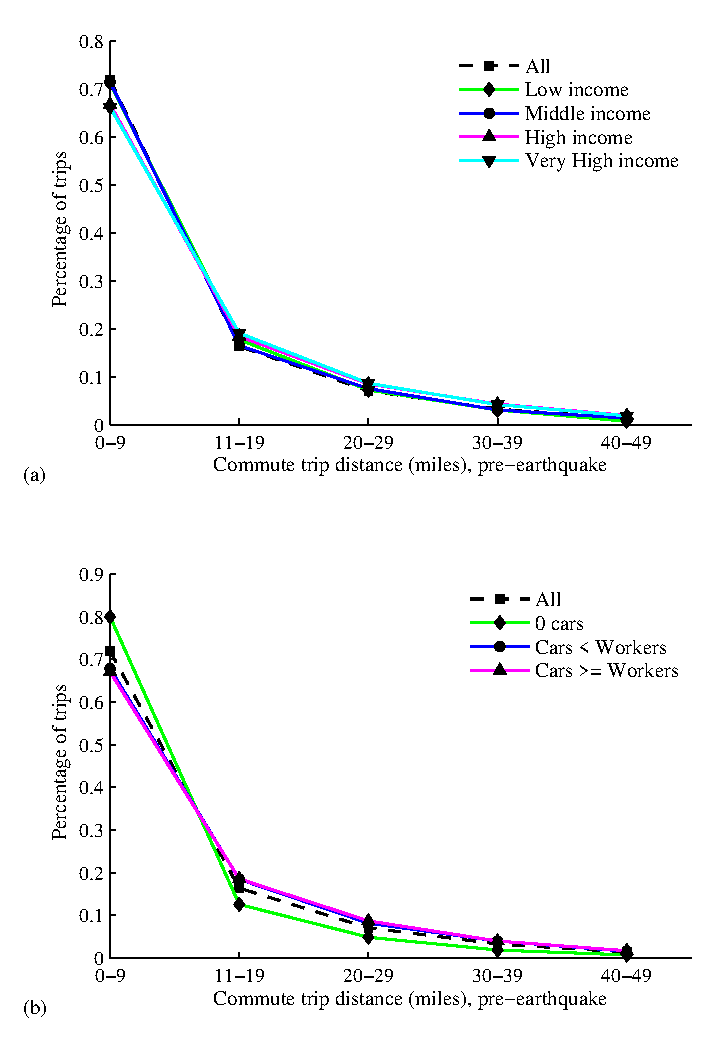
\includegraphics[width=4in]{FIGS/equity_trip_distance_income_cars_to_and_from_work.eps} 
%\caption{Distributions of commute trip length in 10-mile intervals  by a) income class segment, and b) car ownership segment,  (pre-earthquake)}
%\label{fig:lengthIncomeBars}
%\end{figure}

%\subsection{Impact of trip length}
%
\begin{figure}[htb!]
\centering
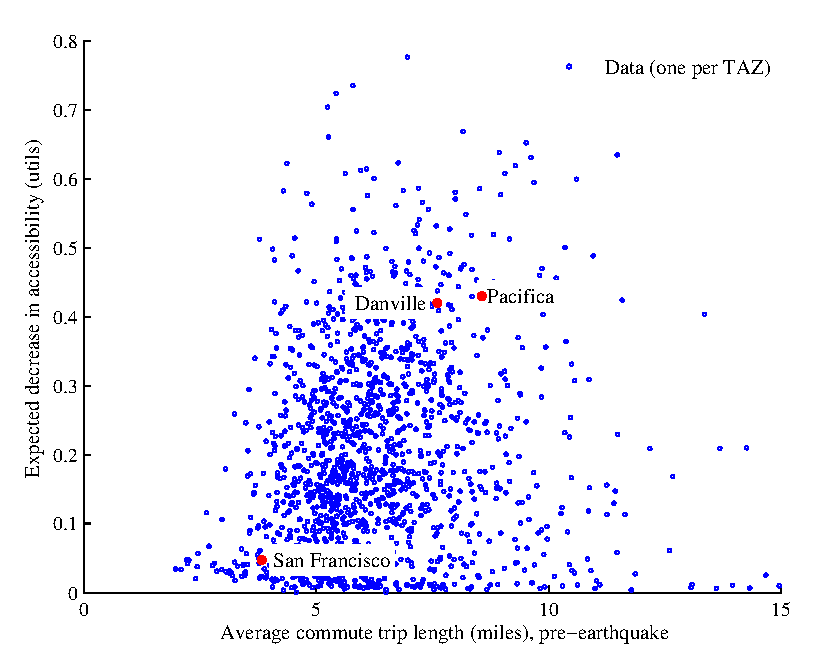
\includegraphics[width=4in]{FIGS/equity_accLengthv4.eps} 
\caption{Average pre-earthquake trip length versus change in expected accessibility for all TAZs in the study region. Each dot represents data from one TAZ, and red dots highlight the data points for the three case study communities.}
\label{fig:accLength}
\end{figure}



Second, controlling for car ownership, we see a fairly consistent distribution of risk across income classes.  For example, looking at households with fewer workers than cars (the middle column of Figure~\ref{fig:acc_by_segment}), the variation from TAZ to TAZ is much greater than the difference across income segments. Similarly, while trip lengths are slightly longer for higher income households, the differences are subtle. % (Figure~\ref{fig:lengthIncomeBars}{(a)}). 
Thus, for a given TAZ, the differences in impacts across incomes are not that great. There is, however, an unequal geographic distribution of wealth in the study region. Because of this, when we aggregate accessibility risk across TAZs, we see that accessibility risk rises slightly with increasing household income  (Figure~\ref{fig:acc_by_TAZ_and_income}{b}). 
%Therefore, even though the poor are generally the most vulnerable to natural disasters,  wealthier households in the San Francisco Bay area are more vulnerable than the other income groups to earthquake-related accessibility risk. [ Jack commented this out--I don't think this conclusion is fully justified. This assumes that greater reduction in accessibility utils is equivalent to greater "vulnerability" in general, but there are a few reasons why this isn't an apples-to-apples comparison.]


%we observe a gradual increase in expected accessibility losses down a column, such as down the right-hand column, representing households where the number of workers is greater than or equal to the number of cars (Figure~\ref{fig:acc_by_segment}{(c,f,i,l)}). However, this trend is more subtle than the trend with car ownership for a fixed income class.




Next, we consider TAZs indicated to have elevated risk.
%: due east of San Francisco, in the suburbs of San Jose, along the coastal and bay-side regions south of San Francisco (e.g., Millbrae and Pacifica), and in parts of San Francisco (south-central neighborhoods including the Westland Highlands and Glen Park neighborhoods). Geographic proximity to hazardous faults is one source of spatial variation. 
The San Francisco Peninsula is at risk of disruption from large magnitude San Andreas earthquakes, while the East Bay is at risk from slightly smaller but more frequent events on the Hayward Fault. Network simulations indicate that both Hayward and San Andreas earthquakes can cause accessibility problems for the East Bay. Figure~\ref{fig:scen_acc} shows realizations of a magnitude 6.85 Hayward event and a magnitude 7.45 San Andreas event---both show high accessibility losses in the East Bay.
%In contrast, the more moderate, more frequent Hayward event caused little impact for San Francisco; the San Andreas events were the chief contributors to the loss of accessibility in San Francisco. 
In contrast, the main predicted accessibility losses in San Francisco correspond primarily to San Andreas events.
Figures~\ref{fig:scen_acc}{c} and~\ref{fig:scen_acc}{d} provide one such example. Figures~\ref{fig:scen_acc}{e} and~\ref{fig:scen_acc}{f} show a lower magnitude event farther away from the main population centers: a magnitude 6.35 event in the Great Valley Pittsburg-Kirby Hills Fault. This shows how the more minor faults in the East Bay can contribute to that area's risk.
%, e.g., Figures~\ref{fig:scen_acc}{(d,f)}. 
%Note that in the three individual earthquake events shown---Hayward, M6.85, b) San Andreas, M7.45, c) San Andreas, M8.25---the accessibility losses are higher than average, since these are major events. 
The Figure~\ref{fig:scen_acc} results are for one specific socio-economic group, but comparable results for the other groups show the same patterns.


%\begin{figure}
%\centering
%\includegraphics[width=\textwidth]{../FIGS/equity_154_198_196.pdf} 
%\caption{Expected changes in accessibility for individual scenarios: a) Hayward, M7.05 (medium income, workers $<$ cars), b) San Andreas, M7.05 (medium income, workers $<$ cars), c) San Andreas, M8.25 (medium income, workers $<$ cars)}
%\label{fig:scen_acc}
%\end{figure}
\begin{figure*}[!htb]
    \centering
        \includegraphics[height=7in]{FIGS/accByEq.pdf}
    \caption{Bridge damage and corresponding accessibility losses by TAZ for medium income households with fewer cars than workers. The top three rows show results from specific events, while the bottom row has expected values calculated as a weighted average over all events.}
    % (the darker the color, the greater the losses). For expected bridge damage, the values are on a continuous scale from white to yellow to red in order of increasing annual likelihood of extensive or complete damage.}
\label{fig:scen_acc}
\end{figure*}


% loss exceedance curve
%Finally, we can examine the rates of loss exceedance. The annual rate, $\lambda$, of exceeding some threshold of network performance, as captured by change in accessibility, is estimated by summing the occurrence rates of all damage maps in which the performance measure exceeds the threshold: 
%\begin{equation}
%\lambda_{X \geq x} = \sum_{j'=1}^{J} w_{j'} \mathbbm{I}(X_{j'}\geq x)
%\label{eq:exceedance}
%\end{equation}
%where $x$ is an accessibility value threshold of interest and $X_{j'}$ is the accessibility value realization for the $j'^{th}$ damage map. The variable $w_{j'}$ is the occurrence rate of the $j'^{th}$ damage map.% ($w_j = \frac{w_j}{c}$ where $c$ is the number of damage map realizations per ground-motion intensity map). 
%%The function $\mathbbm{I}$ is an indicator function that evaluates to 1 if the argument, $x_j' \geq x$, is true and 0 otherwise. 
%The indicator function $\mathbbm{I}$  evaluates to 1 if the argument, $X_{j'} \geq x$, is true, and 0 otherwise.
%By evaluating $\lambda$ at different threshold values, we derive an exceedance curve, Figure~\ref{fig:acc_by_TAZ_and_income}). This graph shows a similar shape to the loss exceedance curves for other performance metrics for this case study network~\cite{miller_seismic_2014}. Note that the results are primarily valid in the 100 to 2475 year return periods, since this is the range chosen for the map selection optimization problem. As a sense of scale, if we use the average value over all TAZs for this 

Finally, we can examine the rates of loss exceedance (eq.~\ref{eq:exceedance}), as shown in Figure~\ref{fig:acc_by_TAZ_and_income}.  %Note these results are primarily valid in the 100 to 2475 year return periods, since this is the range chosen for the map selection optimization problem. %As a sense of scale, if we use the average value over all TAZs for this 
Recognizing that the impact varies significantly by TAZ, as indicated by Figure~\ref{fig:acc_by_segment},
%and the general lognormal shape of the accessibility cumulative distribution functions for a given event (Figure~\ref{fig:xxxx})
we also examine the accessibility loss exceedance curve for three communities: part of the San Francisco Financial District, Danville, and Pacifica. This part of the San Francisco Financial District  represents an area with relatively low expected changes in accessibility, whereas Danville and Pacifica are at an elevated risk in almost all socio-economic groups (Figure~\ref{fig:acc_by_segment}). 
The general trends are corroborated by the loss exceedance curves for these three communities (Figure~\ref{fig:acc_by_TAZ_and_income}{a} shows results for medium income households with fewer cars than workers). The average middle-class person from Danville in a household with fewer cars than workers is expected to experience travel-related losses up to 1 $util$ (or 75 minutes of extra travel time per day) after a rare earthquake. In contrast, a resident of San Francisco's Financial District has expected losses of only a tenth as much when considering the same exceedance rate. At annual rates of less than 0.01 (i.e., return periods greater than 100 years), Danville and Pacifica follow a similar general pattern that differs dramatically from that of San Francisco. 

